% Components and interfaces of the risk_sched + two-queue implementation on OCUDU (README figure).
% Green = this work, white = stock OCUDU. Numbers (1)-(6) are the interfaces of the README table.
% Build: pdflatex fig_components_interfaces.tex
\documentclass[tikz,border=2pt]{standalone}
\usepackage[T1]{fontenc}
\usepackage[utf8]{inputenc}
\usepackage{libertine}
\usepackage[libertine]{newtxmath}
\usetikzlibrary{arrows.meta,calc}

\definecolor{ourfill}{HTML}{DDEFD9}
\definecolor{ourline}{HTML}{2E7D32}
\definecolor{gnbfill}{HTML}{F1F3F5}
\definecolor{boxfill}{HTML}{FFFFFF}
\definecolor{ink}{HTML}{222222}
\definecolor{soft}{HTML}{5F6B76}

\begin{document}
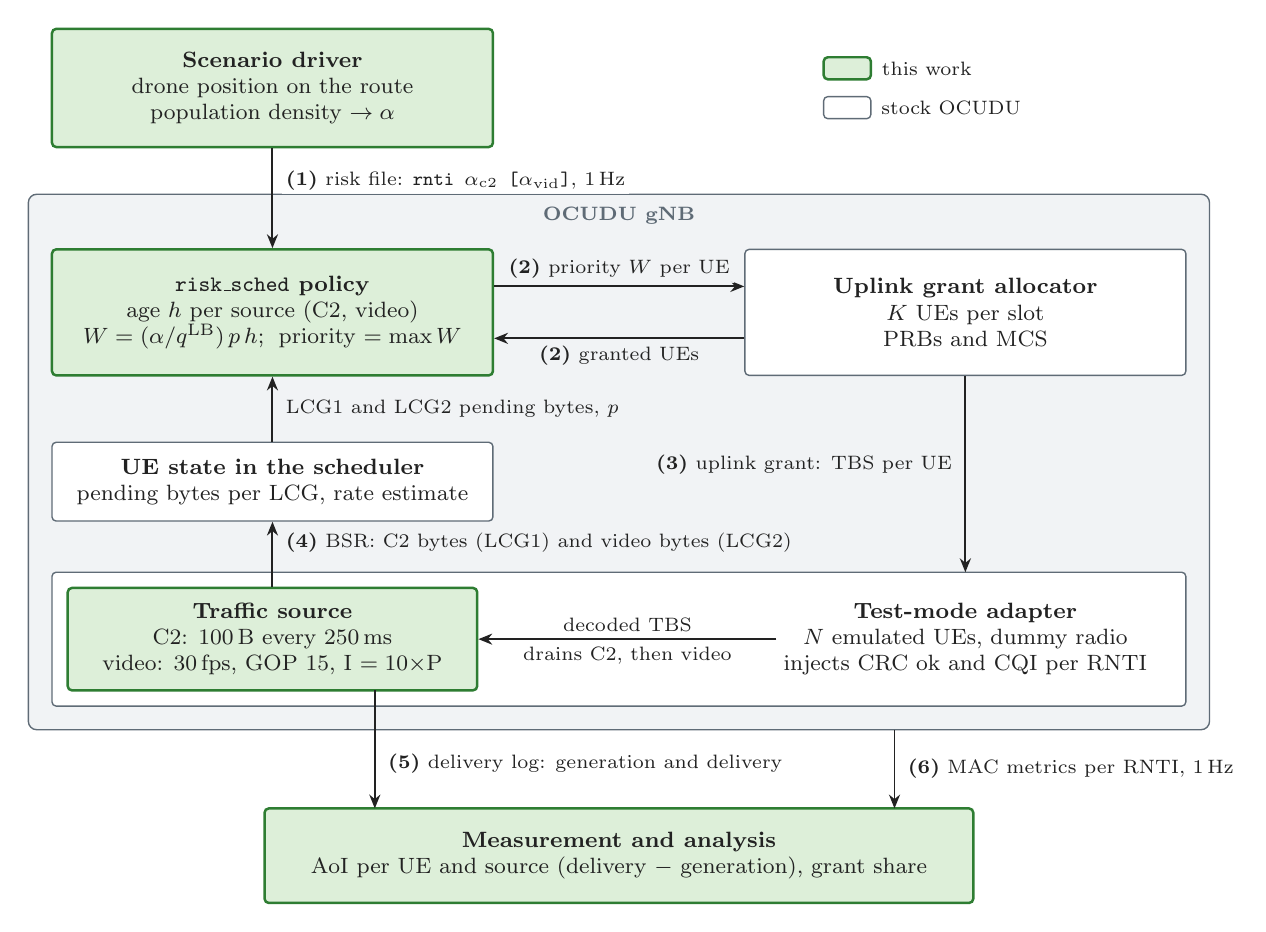
\begin{tikzpicture}[
    x=1cm, y=1cm, font=\footnotesize, text=ink,
    box/.style={line width=0.5pt, rounded corners=1.5pt, align=center, inner sep=3pt},
    stock/.style={box, draw=soft, fill=boxfill},
    ours/.style={box, draw=ourline, fill=ourfill, line width=0.9pt},
    flow/.style={-{Stealth[length=5pt,width=4pt]}, line width=0.7pt, draw=ink},
    lbl/.style={font=\scriptsize, text=ink, inner sep=1.5pt, fill=white, fill opacity=0.92, text opacity=1},
    lblg/.style={lbl, fill=gnbfill},
  ]

  % ---- gNB -------------------------------------------------------------------
  \draw[draw=soft, line width=0.5pt, rounded corners=3pt, fill=gnbfill] (0,2.6) rectangle (15,9.4);
  \node[anchor=north, font=\scriptsize\bfseries, text=soft] at (7.5,9.36) {OCUDU gNB};

  % ---- outside the gNB -----------------------------------------------------------
  \node[ours, minimum width=5.6cm, minimum height=1.5cm] (drv) at (3.1,10.75)
       {\textbf{Scenario driver}\\ drone position on the route\\ population density $\rightarrow \alpha$};
  \node[ours, minimum width=9.0cm, minimum height=1.2cm] (ana) at (7.5,1.0)
       {\textbf{Measurement and analysis}\\ AoI per UE and source (delivery $-$ generation), grant share};

  % ---- inside the gNB ---------------------------------------------------------
  \node[ours, minimum width=5.6cm, minimum height=1.6cm] (pol) at (3.1,7.9)
       {\textbf{\texttt{risk\_sched} policy}\\ age $h$ per source (C2, video)\\
        $W = (\alpha / q^{\mathrm{LB}})\,p\,h$;\; priority $= \max W$};
  \node[stock, minimum width=5.6cm, minimum height=1.6cm] (alloc) at (11.9,7.9)
       {\textbf{Uplink grant allocator}\\ $K$ UEs per slot\\ PRBs and MCS};
  \node[stock, minimum width=5.6cm, minimum height=1.0cm] (st) at (3.1,5.75)
       {\textbf{UE state in the scheduler}\\ pending bytes per LCG, rate estimate};

  % test mode: stock block that hosts our traffic source
  \draw[draw=soft, line width=0.5pt, rounded corners=1.5pt, fill=boxfill] (0.3,2.9) rectangle (14.7,4.6);
  \node[ours, minimum width=5.2cm, minimum height=1.3cm] (src) at (3.1,3.75)
       {\textbf{Traffic source}\\ C2: 100\,B every 250\,ms\\ video: 30\,fps, GOP 15, I $= 10\times$P};
  \node[align=center] (tm) at (11.9,3.75)
       {\textbf{Test-mode adapter}\\ $N$ emulated UEs, dummy radio\\ injects CRC ok and CQI per RNTI};

  % ---- interfaces ------------------------------------------------------------
  \draw[flow] (drv.south) -- node[lbl, pos=0.32, right=3pt]
        {\textbf{(1)} risk file: \texttt{rnti $\alpha_{\mathrm{c2}}$ [$\alpha_{\mathrm{vid}}$]}, 1\,Hz} (pol.north);

  \draw[flow] ([yshift=0.33cm]pol.east) -- node[lblg, above=1pt] {\textbf{(2)} priority $W$ per UE}
              ([yshift=0.33cm]alloc.west);
  \draw[flow] ([yshift=-0.33cm]alloc.west) -- node[lblg, below=1pt] {\textbf{(2)} granted UEs}
              ([yshift=-0.33cm]pol.east);

  \draw[flow] (st.north) -- node[lblg, right=3pt] {LCG1 and LCG2 pending bytes, $p$} (pol.south);

  \draw[flow] (alloc.south) -- node[lblg, pos=0.45, left=3pt] {\textbf{(3)} uplink grant: TBS per UE}
              (alloc.south |- 0,4.6);

  \draw[flow] (9.5,3.75) -- node[lbl, above=1pt] {decoded TBS}
              node[lbl, below=1pt] {drains C2, then video} (src.east);

  \draw[flow] (src.north) -- node[lblg, pos=0.68, right=3pt]
        {\textbf{(4)} BSR: C2 bytes (LCG1) and video bytes (LCG2)} (st.south);

  \draw[flow] (4.4,3.1) -- node[lbl, pos=0.62, right=3pt] {\textbf{(5)} delivery log: generation and delivery}
              (4.4,1.6);
  \draw[flow] (11.0,2.6) -- node[lbl, pos=0.5, right=3pt] {\textbf{(6)} MAC metrics per RNTI, 1\,Hz}
              (11.0,1.6);

  % ---- legend ---------------------------------------------------------------
  \begin{scope}[font=\scriptsize]
    \node[ours,  minimum width=0.6cm, minimum height=0.28cm, inner sep=0pt] (l1) at (10.4,11.0) {};
    \node[anchor=west] at (l1.east) {this work};
    \node[stock, minimum width=0.6cm, minimum height=0.28cm, inner sep=0pt] (l2) at (10.4,10.5) {};
    \node[anchor=west] at (l2.east) {stock OCUDU};
  \end{scope}
\end{tikzpicture}
\end{document}
